\label{chap:optimization}

The objective of the optimization procedure is to refine the inverse model prediction by first reducing the temperature distribution error and subsequently minimizing the process cost. The procedure is designed for practical deployment, allowing direct use by the machine operator through an interface exposing the main control parameters.

The optimization procedure implemented is described in Algorithm~\ref{alg:optimizer}. The algorithm uses the Adam optimizer~\cite{kingma2014adam} for 1000 iterations with a learning rate of $1 \times 10^{-1}$. It takes as input the initial parameter values predicted by $\mathcal{I}$, the maximum allowable temperatures for the top and bottom surfaces of the sheet, denoted by $T_\text{T}^{\max}$ and $T_\text{B}^{\max}$, respectively, the machine-hour cost $h$, and the energy cost $e$. The output of the algorithm is the optimized set of machine parameters $\mathbf{x}^{*}$.

The temperature thresholds, together with the machine-hour and energy costs, can be defined by the machine operator based on the material properties, mold geometry, and the cost optimization objective, such as shorter processing times or reduced energy consumption. Since the optimization is performed at the instance level, these values can be specified more precisely for each case, allowing the optimization to better adapt to the specific problem.


\begin{algorithm}[ht]
	\footnotesize
	\caption{Inverse model process parameters optimization}
	\label{alg:optimizer}
	\begin{algorithmic}[1]
		
		\Require Initial machine parameters $\mathbf{\hat{x}}=\mathcal{I}(\mathbf{\hat{y}})$, maximum allowable temperatures $T_\text{T}^{\max}$ and $T_\text{B}^{\max}$, machine-hour cost $h$ and energy cost $e$
		\Ensure Optimized machine parameters $\mathbf{x}^{*}$
		
		\State $I_1 = 500$
		\label{alg:opt_init_start}
		\State $I_2 = 1000$
		\State Initialize the Adam optimizer
		\State Set $\mathbf{x}^{(0)} \gets \mathbf{\hat{x}}$
		\label{alg:opt_init_end}
		
		\For{$k=1$ to $I_1$} \Comment First stage
		\label{alg:opt_first_start}
		\State $\mathbf{\hat{y}} \gets \mathcal{S}(\mathbf{x}^{(k-1)})$
		\State Extract $\mathbf{\hat{y}}_C$, $\mathbf{\hat{y}}_T$, and $\mathbf{\hat{y}}_B$
		\State Compute $E_T^{\max}$ according to Eq.~\ref{eq:max_temp_error}
		\State Compute $\lambda_\text{T}$ and $\lambda_\text{B}$ according to Eq.~\ref{eq:temperature_penalties}
		\State Evaluate objective function $f_{\text{first}}$ according to Eq.~\ref{eq:f_first}
		\State Update of $\mathbf{x}^{(k)}$ by minimizing $f_{\text{first}}$ with Adam
		\EndFor
		\label{alg:opt_first_end}
		

		\For{$k=I_1$ to $I_2$} \Comment Second stage
		\label{alg:opt_second_start}
		\State $\mathbf{\hat{y}} \gets \mathcal{S}(\mathbf{x}^{(k-1)})$
		\State Extract $\mathbf{\hat{y}}_C$, $\mathbf{\hat{y}}_T$, and $\mathbf{\hat{y}}_B$
		\State Compute $E_T^{\max}$ according to Eq.~\ref{eq:max_temp_error}
		\State Compute $\lambda_\text{T}$ and $\lambda_\text{B}$ according to Eq.~\ref{eq:temperature_penalties}
		\State Evaluate objective function $f_{\text{first}}$ according to Eq.~\ref{eq:f_first}
		\State Compute $\sigma$ according to Eq.~\ref{eq:tradeoff_sigmoid}
		\State Evaluate objective function $f_{\text{second}}$ according to Eq.~\ref{eq:f_second}
		\State Update of $\mathbf{x}^{(k)}$ by minimizing $f_{\text{second}}$ with Adam
		\EndFor
		\label{alg:opt_second_end}
		
		\State $\mathbf{x}^{*} \gets \mathbf{x}^{(1000)}$
		\label{alg:opt_output_start}
		\State \textbf{return} $\mathbf{x}^{*}$
		\label{alg:opt_output_end}
		
	\end{algorithmic}
\end{algorithm}

The optimization algorithm is divided into two stages of 500 iterations each. The first stage focuses on reducing the temperature distribution error using Eq.~\ref{eq:f_first} as the objective function. The second stage aims to minimize the process cost while preserving the temperature accuracy achieved in the first stage, using Eq.~\ref{eq:f_second} as the objective function.

In the first-stage of the optimization, during the initialization in lines~\ref{alg:opt_init_start}--\ref{alg:opt_init_end} of Algorithm~\ref{alg:optimizer}, the Adam optimizer is initialized, and the machine parameters predicted by the inverse model $\mathbf{\hat{x}}$, are set as the starting point of the optimization. 

As illustrated in lines~\ref{alg:opt_first_start}--\ref{alg:opt_first_end} of Algorithm~\ref{alg:optimizer}, the surrogate model $\mathcal{S}$ is evaluated for the current machine parameters, and the resulting output prediction are used to compute the temperature error. 

The temperature error considered is computed as the maximum absolute deviation between the predicted and target temperature distributions, incorporating a tolerance margin $\epsilon = 3~^\circ\mathrm{C}$, consistently with the error formulation used in the inverse model (see Section~\ref{sec:inverse_loss_function}):

\begin{equation}
	E_T^{\text{max}} = \max \left| \mathbf{\hat{y}}_C - \left(\mathbf{y}_C + \frac{\epsilon}{2}\right) \right|
\label{eq:max_temp_error}
\end{equation}

\noindent overheating is penalized when the predicted top and bottom temperatures exceed the allowable limits:
\begin{equation}
	\lambda_\text{T} = \max(\mathbf{\hat{y}}_\text{T} - T_\text{T}^{\max}, 0), \quad
	\lambda_\text{B} = \max(\mathbf{\hat{y}}_\text{B} - T_\text{B}^{\max}, 0)
	\label{eq:temperature_penalties}
\end{equation}

The first-stage optimization objective function is defined as:
\begin{equation}
	f_{\text{first}} = E_T^{\text{max}} + \lambda_\text{T} + \lambda_\text{B}.
	\label{eq:f_first}
\end{equation}

During the second stage of the optimization, as reported in lines~\ref{alg:opt_second_start}--\ref{alg:opt_second_end} of Algorithm~\ref{alg:optimizer}, the output obtained from the first-stage is used as the initial input. In this case the objective is to reduce the process cost while preserving the temperature accuracy achieved at the end of the first stage. To this end, a sigmoid function is used to modulate the trade-off between temperature accuracy and process cost minimization:

\begin{equation}
	\sigma = \text{sigmoid} \left( \frac{E_T^{\text{max}} - \epsilon}{\tau \cdot \epsilon} + \lambda_\text{T} + \lambda_\text{B} \right)
	\label{eq:tradeoff_sigmoid}
\end{equation}

The objective function minimized during the second stage is:
\begin{equation}
	f_{\text{second}} = \sigma f_{\text{first}} - (1 - \sigma) \cdot \frac{1}{P_{\text{Cost}}} - \epsilon.
	\label{eq:f_second}
\end{equation}

\noindent where $P_{\text{Cost}}$ is the cost function defined in Eq.~\ref{eq:cost}.

Finally, after completion of the two optimization stages, the resulting machine parameters are returned, as reported in lines~\ref{alg:opt_output_start}--\ref{alg:opt_output_end} of Algorithm~\ref{alg:optimizer}. 

%Unlike the neural network models, which are trained using fixed average cost coefficients across all samples, this formulation allows the machine operator to adjust the relative importance of the cost components $h$ and $e$ in Eq.~\ref{eq:cost} at inference time for each instance, enabling different operational objectives, such as shorter processing times or reduced energy consumption.


\section{Evaluation}

To evaluate the effectiveness of the inverse model initialization, we compare the maximum absolute temperature error obtained after optimization when initialized with the parameters predicted by $\mathcal{I}$ against a random initialization. The analysis is conducted using paired comparisons on both validation and test sets, in order to assess the behavior of the optimizer on both simulated and real data.

The results were obtained by executing the optimization strategy, taking into account the material-specific thresholds indicated in~\cite{schwarzmann2018thermoforming} when selecting the maximum allowable temperatures $T_\text{T}^{\max}$ and $T_\text{B}^{\max}$. To allow for comparison with the results obtained from the inverse model, the values of $h$ and $e$ in Eq.~\ref{eq:cost} were set to the same values used by the inverse model and kept constant across all examples.

On the validation set, initialization from the inverse model yields a lower maximum absolute error than random initialization in 80\% of the cases, with a statistical significance of $p_{value} = 9.132e-54$, computed using the \emph{Wilcoxon signed-rank test}~\cite{woolson2007wilcoxon}. On the test set, this proportion is 67\%, with $p_{value} = 3.015e-5$.

These results indicate that initialization from the inverse model provides a more favorable starting point for the optimization procedure than random initialization. Specifically, after the optimization procedure starting form the inverse model outputs, we achieved a maximum average absolute error of $3.15^\circ\mathrm{C}$ on the validation set and $4.23^\circ\mathrm{C}$ on the test set.

\begin{figure}[t]
	\centering
	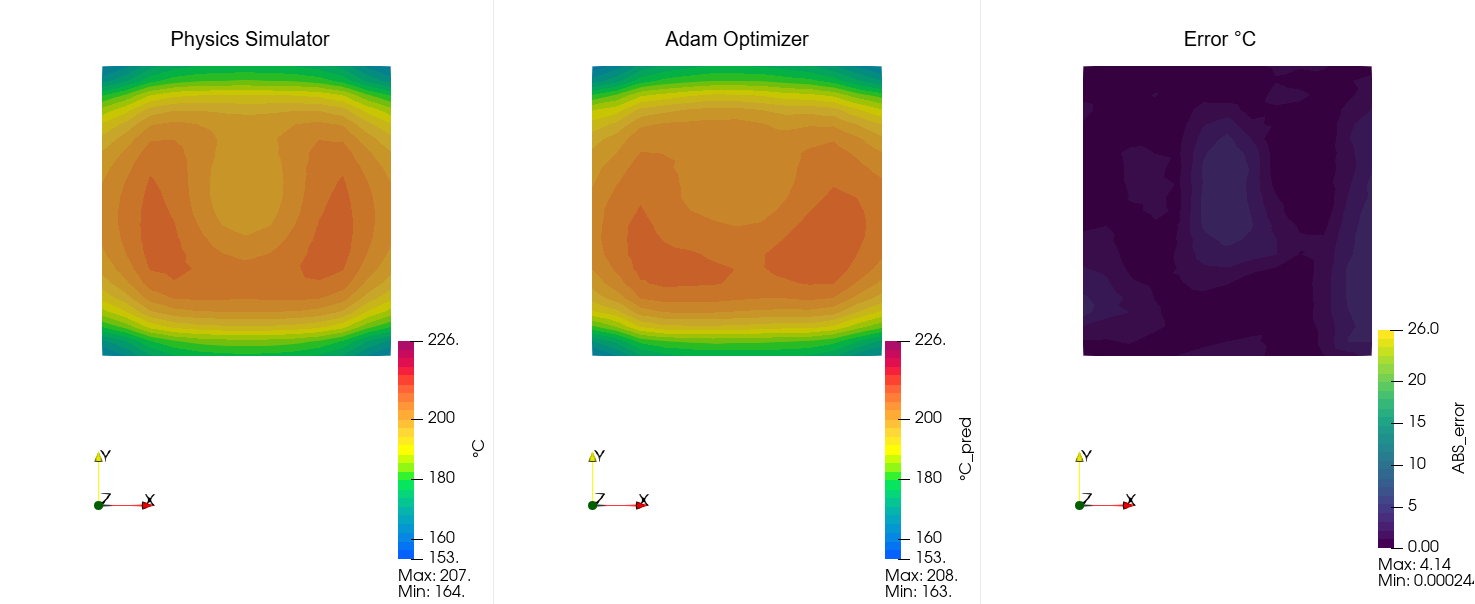
\includegraphics[width=0.7\linewidth]{figures/adam_optimizer_with_label.png}
	\caption{Prediction example on the test set. From left to right: the temperature distribution obtained from the physics-based simulator, the prediction produced by the optimizer, and the absolute error between the target temperature distribution and the predicted one.}
	\label{fig:optimizer_prediction}
\end{figure}

Figure~\ref{fig:optimizer_prediction} illustrates the same example shown in Figure~\ref{fig:surrogate_model_prediction} and Figure~\ref{fig:inverse_model_prediction}, considering the prediction obtained after optimization. The error previously observed along the right-hand side of the sheet is significantly reduced, while the remaining deviations are mainly concentrated in the central region, where the predicted temperature is slightly higher than the target.

The optimizer maintains the tendency to favor higher heating power over shorter durations, reflecting the trade-off learned by the inverse model between energy consumption and processing time. However, compared to the inverse model, the optimization step places greater emphasis on reducing the temperature distribution error by allowing longer heating times. As a result, the additional cost reduction is smaller than that achieved by the inverse model, with a reduction of 11.77\% on the validation set and 8.98\% on the test set.



